\documentclass[border=10pt]{standalone}
\usepackage{tikz}
\usetikzlibrary{arrows.meta,calc}
\definecolor{cwork}{RGB}{72,116,158}
\definecolor{csetup}{RGB}{86,156,104}
\definecolor{crepair}{RGB}{198,86,76}
\definecolor{cpm}{RGB}{222,158,74}
\begin{document}
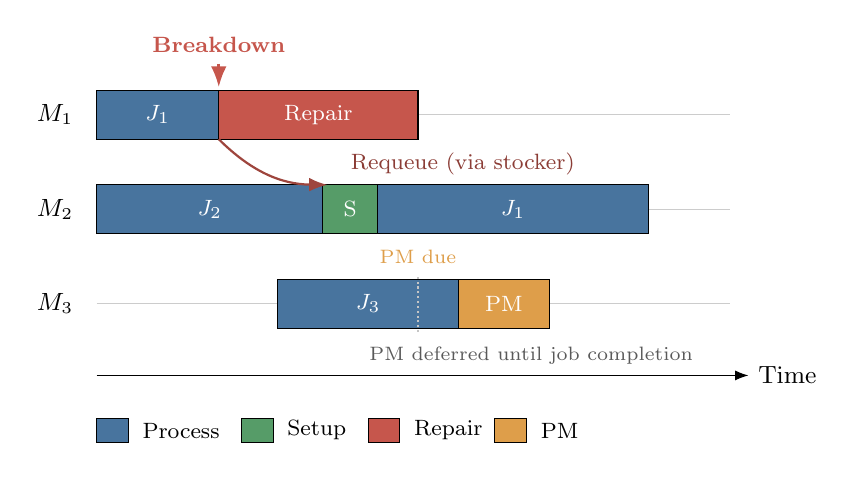
\begin{tikzpicture}[font=\small,>=Latex,x=1.15cm,y=1cm]
  \def\h{0.62}
  % bar: \gbar{x1}{x2}{yrow}{color}{label}
  \newcommand{\gbar}[5]{\fill[#4] (#1,#3) rectangle (#2,#3+\h);
     \draw (#1,#3) rectangle (#2,#3+\h);
     \node[font=\footnotesize,text=white] at ({(#1+#2)/2},#3+\h/2) {#5};}
  % rows
  \def\Ma{3.3}\def\Mb{2.1}\def\Mc{0.9}
  \foreach \y/\m in {\Ma/$M_1$,\Mb/$M_2$,\Mc/$M_3$} {
     \node[anchor=east] at (-0.15,\y+\h/2) {\m};
     \draw[gray!40] (0,\y+\h/2) -- (7.0,\y+\h/2);
  }
  % M1: J1 interrupted partway (failed process), then Repair
  \gbar{0}{1.35}{\Ma}{cwork}{$J_1$}
  \gbar{1.35}{3.55}{\Ma}{crepair}{Repair}
  % M2: J2, Setup (type change), J1 resumed = full process time
  \gbar{0}{2.5}{\Mb}{cwork}{$J_2$}
  \gbar{2.5}{3.1}{\Mb}{csetup}{S}
  \gbar{3.1}{6.1}{\Mb}{cwork}{$J_1$}
  % M3: J3, then PM (shorter than repair)
  \gbar{2.0}{4.0}{\Mc}{cwork}{$J_3$}
  \gbar{4.0}{5.0}{\Mc}{cpm}{PM}
  % --- breakdown marker on M1 (mid-process) ---
  \draw[crepair,line width=1.0pt,->] (1.35,\Ma+\h+0.34) -- (1.35,\Ma+\h+0.04);
  \node[crepair,font=\footnotesize\bfseries,anchor=south] at (1.35,\Ma+\h+0.36) {Breakdown};
  % --- requeue arrow M1 -> M2 (J1 requeued via stocker) ---
  \draw[->,thick,crepair!80!black] (1.35,\Ma) to[bend right=22] (2.55,\Mb+\h);
  \node[font=\footnotesize,crepair!70!black,anchor=west] at (2.7,2.98) {Requeue (via stocker)};
  % --- PM-due marker on M3 (reached during J3, deferred) ---
  \draw[gray!45,densely dotted,line width=0.75pt] (3.55,\Mc-0.05) -- (3.55,\Mc+\h+0.06);
  \node[font=\scriptsize,anchor=south,text=cpm] at (3.55,\Mc+\h+0.08) {PM due};
  \node[font=\scriptsize,anchor=north,align=center,text=black!65] at (4.8,\Mc-0.12) {PM deferred until job completion};
  % --- time axis ---
  \draw[->] (0,0.3) -- (7.2,0.3) node[right]{Time};
  % --- legend ---
  \begin{scope}[shift={(0,-0.55)}]
    \foreach \i/\c/\t in {0/cwork/Process, 1.6/csetup/Setup, 3.0/crepair/Repair, 4.4/cpm/PM} {
      \fill[\c] (\i,0) rectangle (\i+0.35,0.3); \draw (\i,0) rectangle (\i+0.35,0.3);
      \node[anchor=west,font=\footnotesize] at (\i+0.4,0.15) {\t};
    }
  \end{scope}
\end{tikzpicture}
\end{document}
